% ======================================================================
% PropPulse — Project Review 1 Report
% Compile:  pdflatex main.tex  (twice, for references)
% Figures are referenced relative to this file (../../figures/*.png).
% If you upload to Overleaf, upload the figures/ folder next to main.tex
% and replace ../../figures/ below with figures/  (or set \graphicspath).
% ======================================================================
\documentclass[11pt,a4paper]{article}

\usepackage[margin=2.4cm]{geometry}
\usepackage{graphicx}
\usepackage{booktabs}
\usepackage{float}
\usepackage{caption}
\usepackage{xcolor}
\usepackage[hidelinks]{hyperref}
\usepackage{url}

\definecolor{propnavy}{HTML}{1F3864}
\captionsetup{font=small,labelfont={bf,color=propnavy}}

\title{\textcolor{propnavy}{\textbf{PropPulse}}\\[4pt]
\large ML-Driven Property Valuation \& Market Intelligence\\
for Residential Real Estate\\[10pt]
\normalsize Project Review 1 --- Problem Statement, Abstract \& EDA}
\author{%
\begin{tabular}{ll}
\textbf{Rushmanth Nalluri} & 2500030215 \\
\textbf{Sk Mastan Saheb} & 2500030370 \\
\textbf{Rayala Deepak} & 2500030717 \\
\end{tabular}\\[12pt]
Under the guidance of \textbf{Guide Name, Designation}\\
Department of Computer Science \& Engineering, Institute Name}
\date{August 2026}

\begin{document}
\maketitle
\thispagestyle{empty}

\begin{center}
\small Repository: \url{https://github.com/rushmanthnalluri/prop-pulse} \quad
(branch \texttt{main}) \quad$\cdot$\quad Dataset: Ames, Iowa (Kaggle)
\end{center}

% ====================================================================
\begin{abstract}
\noindent
PropPulse is an end-to-end machine-learning platform for residential property
valuation in Ames, Iowa, built on the Kaggle \emph{House Prices: Advanced
Regression Techniques} dataset (1{,}460 sales, 2006--2010). The problem
addressed is the opacity of residential property pricing: buyers, sellers and
agents lack estimates that are simultaneously accurate and explainable. Given
the attributes of a property, the system predicts (i)~its sale price ---
regression on $\log(1+\text{SalePrice})$ served back in dollars with an
$\sim$80\% prediction interval, (ii)~the probability that it sells within
30~days --- calibrated classification, and (iii)~its micro-market segment ---
DBSCAN clustering of the 25 Ames neighbourhoods. Every prediction is explained
with per-prediction SHAP factors and served through a FastAPI backend consumed
by a React dashboard, with MLflow experiment tracking, PSI drift monitoring,
and Docker packaging. The methodology is leakage-safe by construction: a
time-based split (train $\le$~2008 / validation 2009 / sealed test 2010), all
aggregate statistics fit on the train split only, and a single feature pipeline
shared by training and serving. This review presents the problem statement and
abstract, and reports the completed exploratory data analysis: a fully
executed, reproducible notebook producing 14 figures, with all code, data
artifacts, and design decisions (ADRs) versioned in the project git repository.
\end{abstract}

% ====================================================================
\section{Problem Statement}
Residential property pricing is opaque. Market participants rely on rules of
thumb, and widely used online estimates rarely explain \emph{why} a home is
worth what it is. The goal of this project is: \textbf{given the attributes of
a residential property in Ames, Iowa, build a machine-learning system that
estimates}
\begin{enumerate}
  \item \textbf{sale price} (regression), with a prediction interval, reported
        in dollars;
  \item \textbf{probability of selling within 30 days} (calibrated
        classification); and
  \item \textbf{micro-market segment} (unsupervised clustering of the 25
        neighbourhoods),
\end{enumerate}
where every estimate is \textbf{explainable} (per-prediction SHAP factors) and
served through a usable product --- an API plus an interactive dashboard ---
rather than a stand-alone notebook.

% ====================================================================
\section{Objectives and Scope}
\begin{itemize}
  \item \textbf{O1 --- Data pipeline:} ingest $\rightarrow$ clean $\rightarrow$
        validate $\rightarrow$ time-based split (945 / 338 / 175 rows).
        \hfill\emph{[done]}
  \item \textbf{O2 --- EDA:} 14-figure reproducible analysis of the train
        split --- the subject of this review. \hfill\emph{[done]}
  \item \textbf{O3 --- Feature engineering:} 94 model features from one
        pipeline shared by training and serving.
  \item \textbf{O4 --- Modelling:} 5 regression + 4 classification candidates;
        champion selection on validation; DBSCAN micro-markets.
  \item \textbf{O5 --- Explainability:} global and per-prediction SHAP.
  \item \textbf{O6 --- Product:} FastAPI backend, React dashboard, drift
        monitoring, Docker, CI and automated tests.
\end{itemize}
Scope boundaries, stated honestly: one city, 1{,}460 labelled rows, sales from
2006--2010. The raw data has two documented gaps, each covered by an explicit,
labelled fallback (ADRs in the repository): no per-property coordinates
$\rightarrow$ approximate neighbourhood centroids; no days-on-market
$\rightarrow$ a transparent, seeded simulation whose classification metrics are
never presented as real-world performance. The test split (2010) remains sealed
until final evaluation.

% ====================================================================
\section{Dataset}
The dataset is the Kaggle \emph{House Prices: Advanced Regression Techniques}
archive --- residential sales in Ames, Iowa, 2006--2010, compiled by
De~Cock~\cite{decock2011}. The labelled file holds 1{,}460 rows $\times$ 81
columns (the competition test file has no \texttt{SalePrice} and is never used
for evaluation). Features cover size, quality/condition, age, amenities,
neighbourhood and sale period.

\begin{itemize}
  \item \textbf{Time-based split (no shuffling):} train = sales $\le$ 2008
        (945 rows), validation = 2009 (338), test = 2010 (175, sealed).
  \item \textbf{Cleaning} follows the official data description: most missing
        values are \emph{structural} (``feature absent'') and are filled as
        \texttt{"None"}; only \texttt{LotFrontage} is genuinely imputed, using
        train-fit neighbourhood medians.
  \item \textbf{Outliers:} exactly two partial-sale rows removed on train
        (Ids 524, 1299); the 39 high-price rows above the IQR fence are genuine
        luxury stock and are kept.
  \item \textbf{Headline (train, $n=945$):} median price \$164{,}990, mean
        \$182{,}125, range \$35{,}311--\$755{,}000; 25 neighbourhoods with a
        3.18$\times$ median-price spread.
\end{itemize}

% ====================================================================
\section{Exploratory Data Analysis}
The EDA is performed on the processed \textbf{train split only}
($945 \times 85$; the sealed test split was never opened) and is fully
reproducible: \texttt{notebooks/01\_eda.ipynb} executes 16/16 cells with zero
errors and regenerates all 14 figures in \texttt{figures/}. Key findings
follow; the full report is \texttt{reports/EDA\_REPORT.md} in the repository.

\subsection{Target distribution: right-skewed, log transform mandatory}
Raw \texttt{SalePrice} is strongly right-skewed (skewness 1.967, excess
kurtosis 7.55); the mean sits $\sim$10\% above the median due to a premium tail
reaching \$755{,}000. After $\log(1+x)$ the distribution is near-symmetric
(skewness 0.175, kurtosis 0.82) --- Figure~\ref{fig:target}. Since errors
scale with price, we train on $\log(1+\text{SalePrice})$, use RMSLE as the
primary metric, and report dollars via $\exp(x)-1$.

\begin{figure}[H]
  \centering
  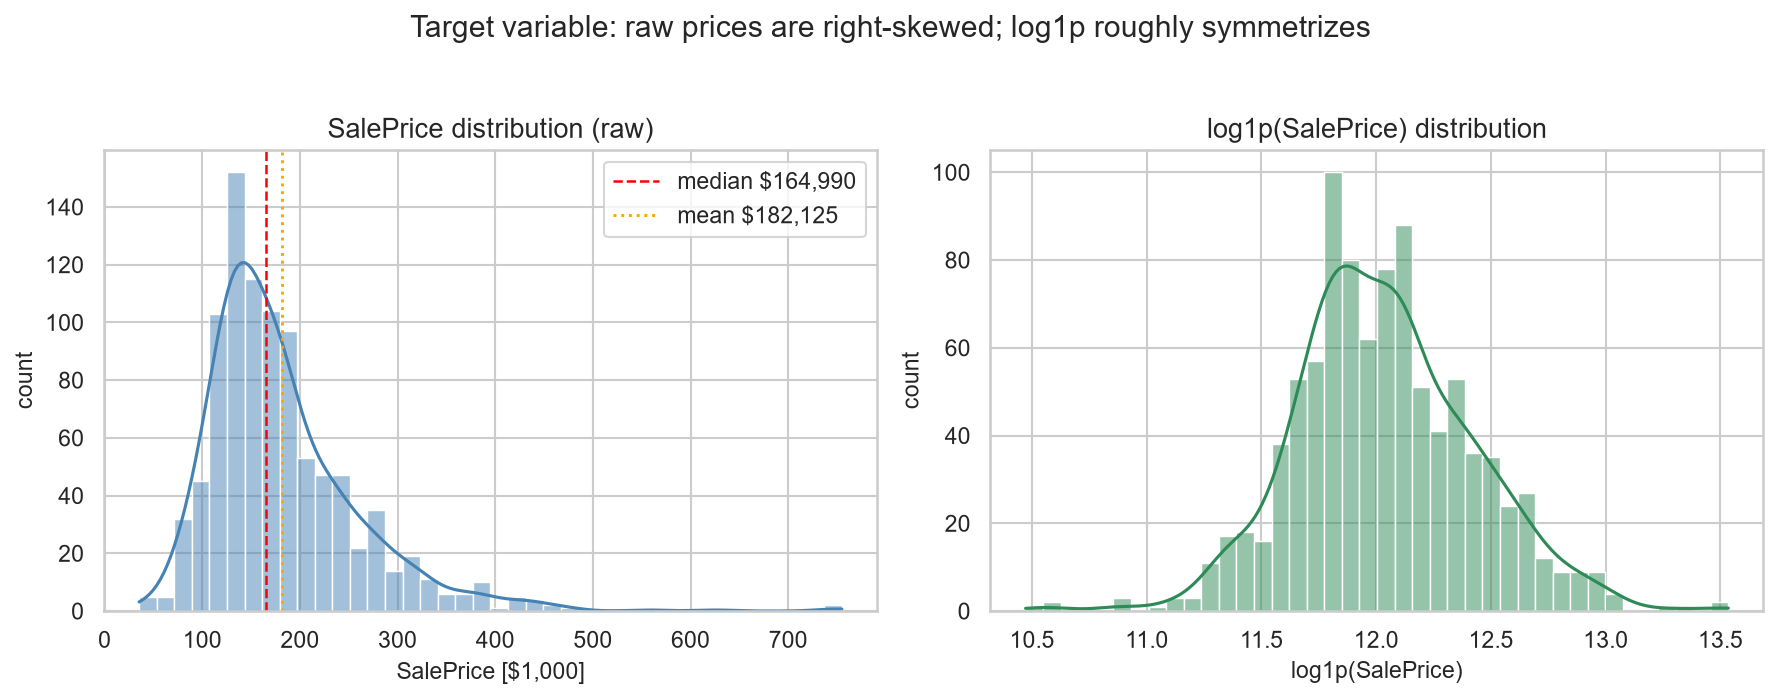
\includegraphics[width=0.86\textwidth]{../../figures/01_saleprice_distribution.png}
  \caption{SalePrice before/after \texttt{log1p}: skewness 1.967 $\to$ 0.175.}
  \label{fig:target}
\end{figure}

\subsection{What drives price}
\textbf{OverallQual is the single strongest feature} (Pearson $r=0.789$):
median price climbs from \$109{,}454 (grade 4) to \$465{,}750 (grade 10) ---
an approximately exponential ladder in dollars, further supporting the log
target. The size block follows (GrLivArea 0.752, TotalBsmtSF 0.639,
\texttt{total\_bath} 0.636, GarageCars 0.634), and the engineered
\texttt{amenity\_count} already reaches $r=0.609$. Property age is negatively
correlated ($r=-0.493$) but non-monotone at the old end (surviving character
homes). Multicollinearity inside the size block is heavy
(GarageCars$\leftrightarrow$GarageArea 0.89) --- tree ensembles or regularized
linear models absorb it, and feature importance must be read in groups.
Figure~\ref{fig:heatmap} shows the correlation structure; price per square
foot (median \$120.58, skew 0.434) is tight, confirming most raw-price skew is
a \emph{size} effect, not a price-level effect.

\begin{figure}[H]
  \centering
  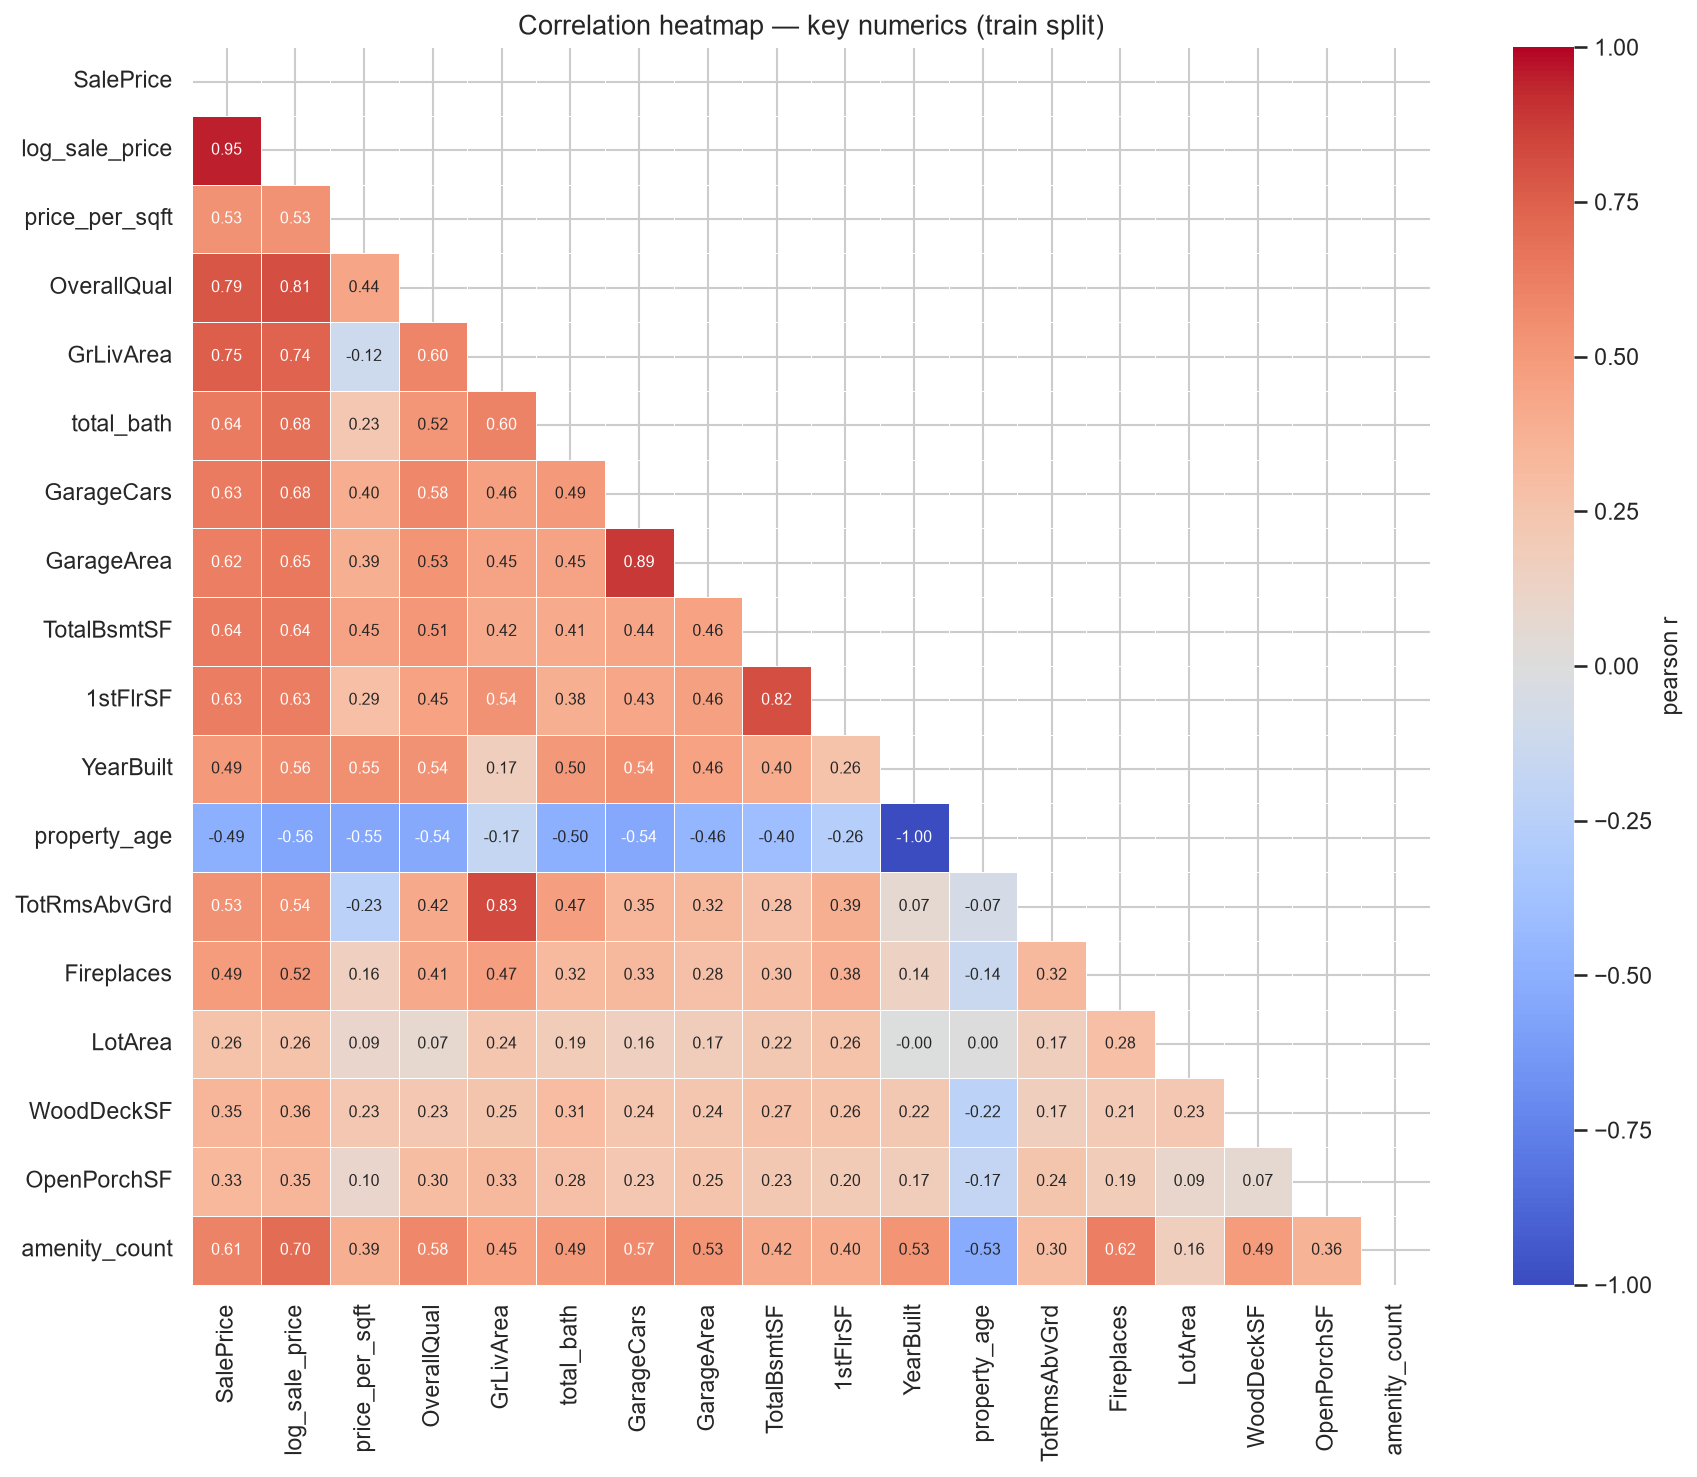
\includegraphics[width=0.7\textwidth]{../../figures/11_correlation_heatmap.png}
  \caption{Masked Pearson correlation heatmap of the key numeric features.}
  \label{fig:heatmap}
\end{figure}

\subsection{Location: neighbourhood identity is the signal}
Median prices span \textbf{3.18$\times$} across the 25 neighbourhoods ---
NridgHt \$318{,}000 vs.\ BrDale \$100{,}000 (Figure~\ref{fig:nbhd}). Premium
\$/sqft concentrates in the north/northwest (NridgHt, NoRidge, StoneBr), while
distance to downtown correlates only weakly with price ($r=+0.279$). Location
value therefore lives in \emph{neighbourhood identity}, not radial distance ---
this justifies both the train-only neighbourhood statistics and DBSCAN
micro-market clustering. Rare neighbourhoods (Blueste $n=1$, NPkVill $n=3$)
carry noisy statistics, a noted caution.

\begin{figure}[H]
  \centering
  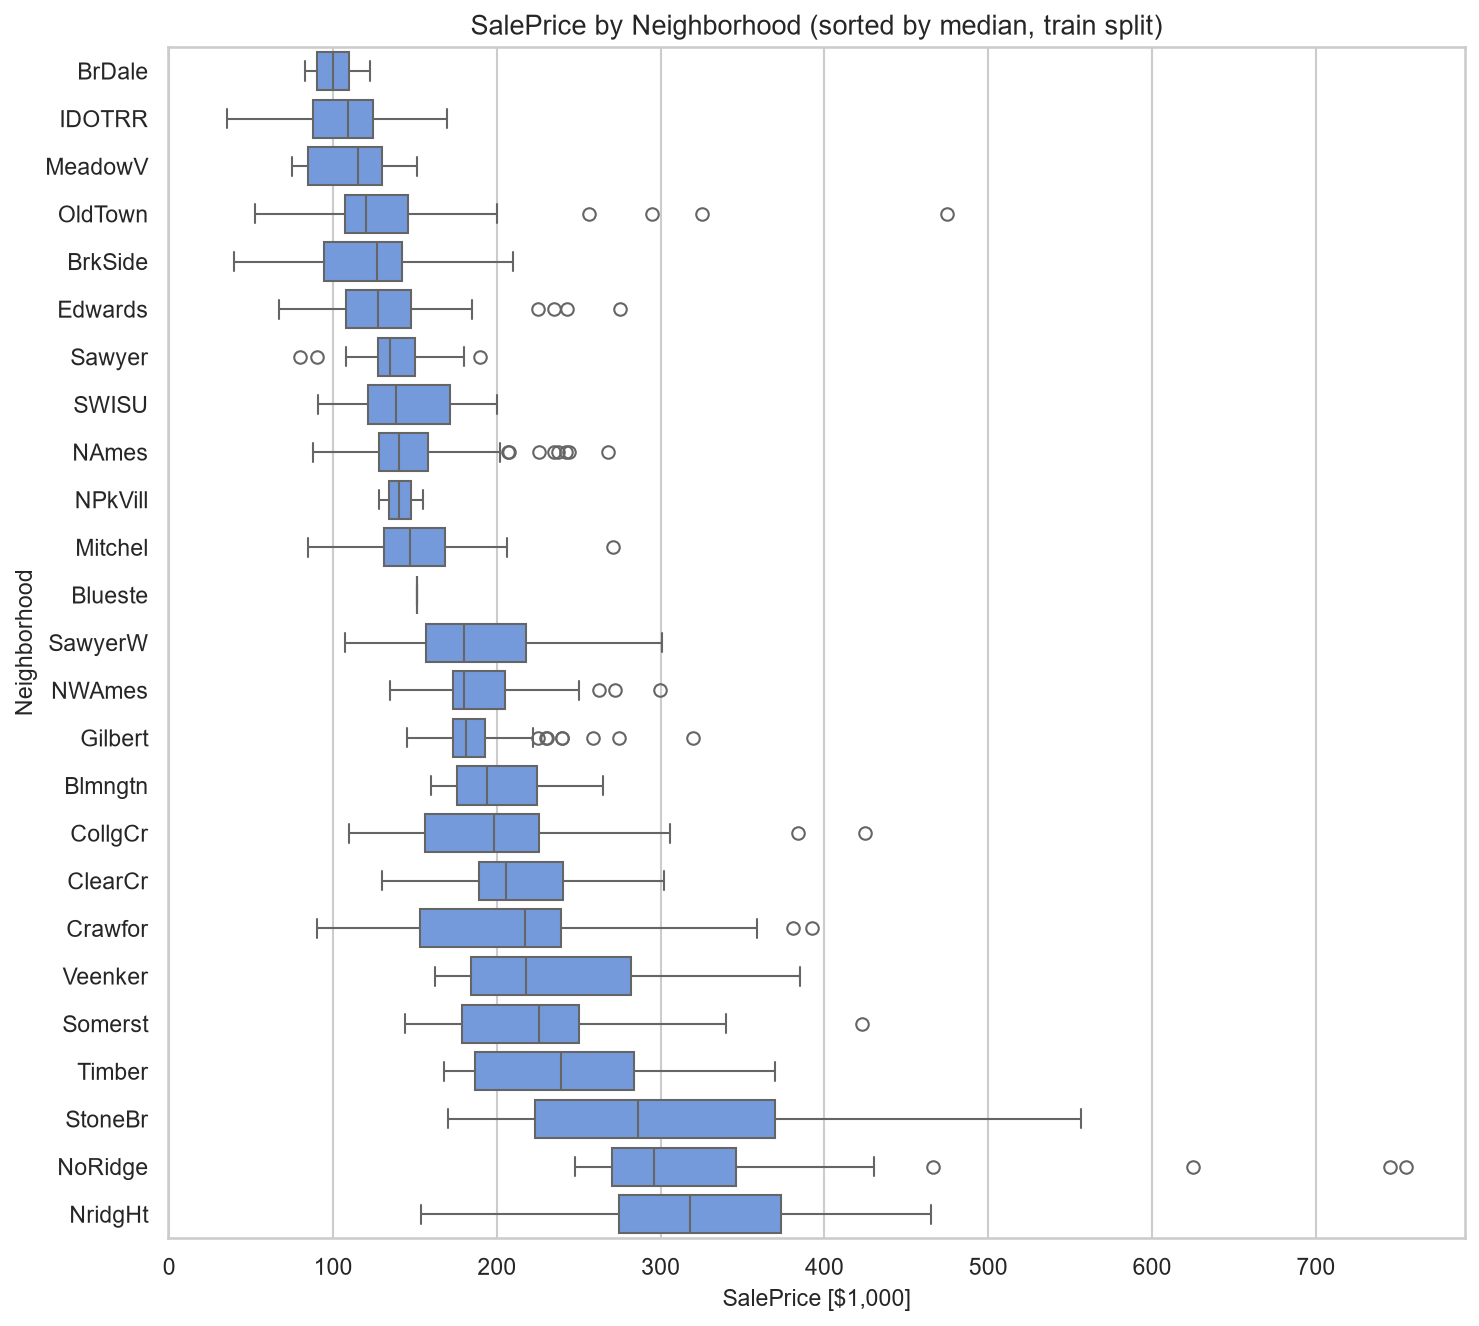
\includegraphics[width=0.82\textwidth]{../../figures/09_neighborhood_prices.png}
  \caption{All 25 neighbourhoods sorted by median price: a 3.18$\times$ spread.}
  \label{fig:nbhd}
\end{figure}

\subsection{Data quality: missingness and outliers}
19 of 81 raw columns contain missing values, but nearly all are
\emph{structural} (PoolQC 99.5\%, MiscFeature 96.3\%, Alley 93.8\% --- the
feature is absent, per the data description) and are filled as \texttt{"None"},
not imputed; only \texttt{LotFrontage} (17.7\%) is a genuine measurement gap,
imputed with train-fit neighbourhood medians. Outlier analysis removes exactly
two rows on train (Ids 524, 1299 --- verified \texttt{SaleCondition~=~Partial}
sales far below size-predicted price). No further trimming: the 39 rows above
the price IQR fence are genuine luxury stock, and the log target plus tree
models already handle the tail.

\begin{figure}[H]
  \centering
  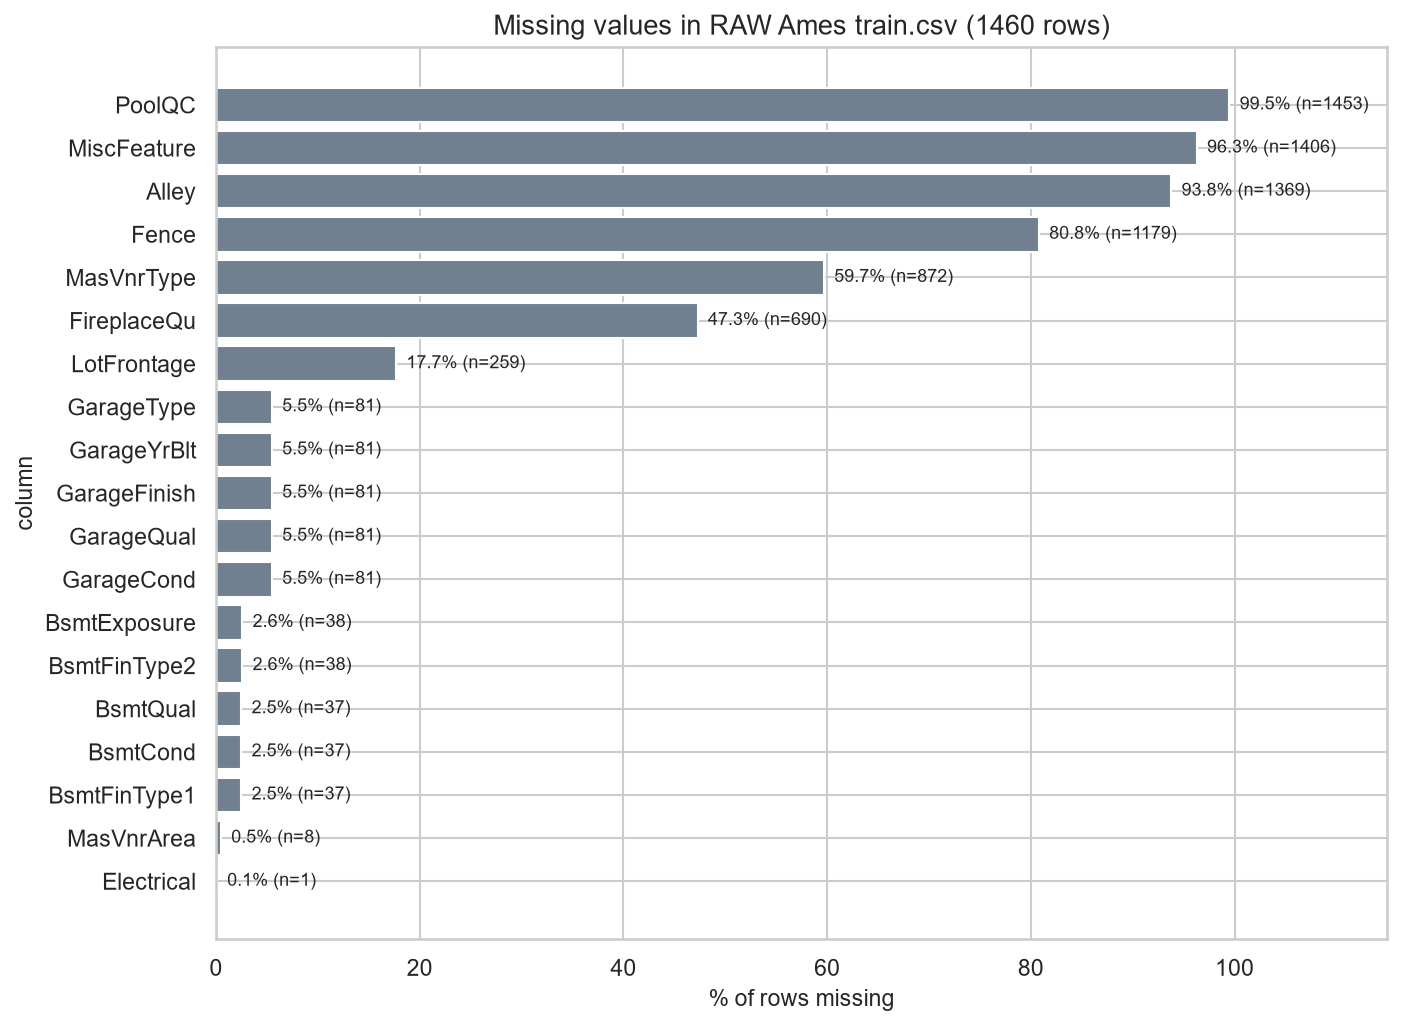
\includegraphics[width=0.72\textwidth]{../../figures/12_missingness_raw.png}
  \caption{Raw-data missingness: 19 columns, almost all structural NAs.}
  \label{fig:missing}
\end{figure}

\subsection{Seasonality and the (simulated) sale-speed target}
Sales \emph{volume} is strongly seasonal --- July peak (167 sales) vs.\
February trough (27) --- while the median price by month moves far less; yearly
median price 2006$\to$2008 changed only $+0.6\%$, so the time-based split
faces no distribution shock at its boundary. The days-on-market target is a
documented, seeded \textbf{simulation} (ADR-3): median 41 days, 25.3\% of sales
``fast'' ($\le$30 days). All classification metrics are labelled accordingly,
and modelling must be class-imbalance-aware (class weights, PR-AUC primary).

\begin{figure}[H]
  \centering
  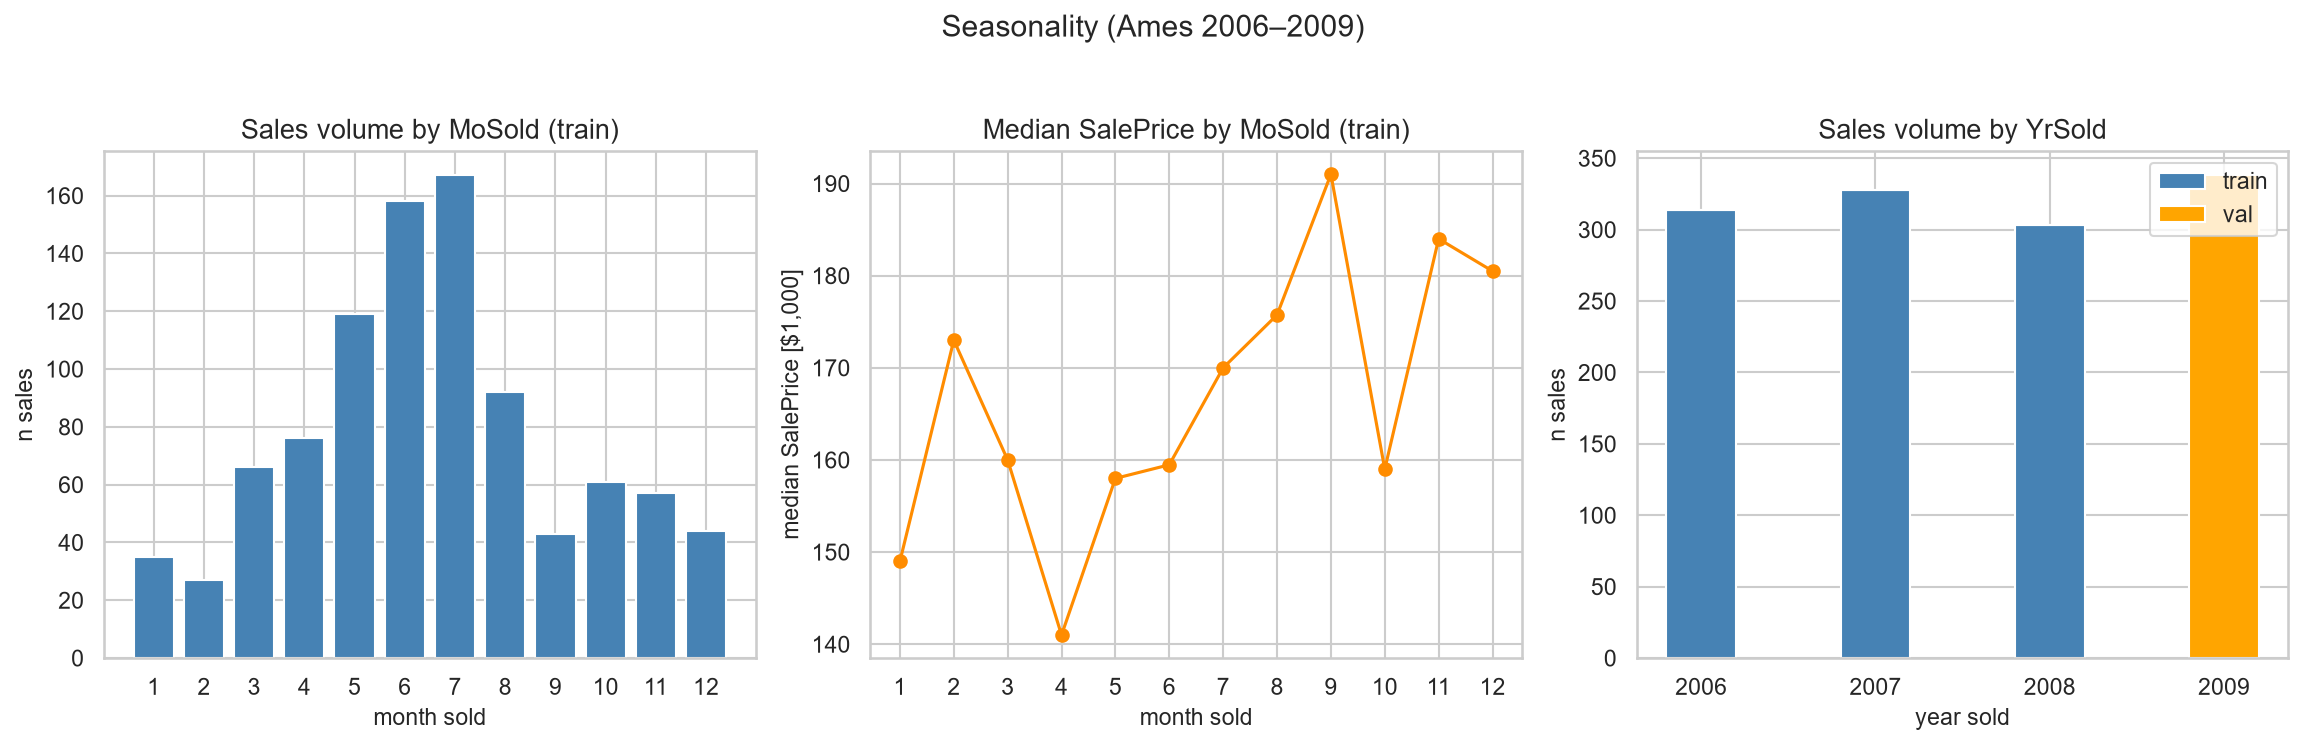
\includegraphics[width=0.78\textwidth]{../../figures/14_seasonality.png}
  \caption{Seasonality: strong volume cycle, nearly flat price level.}
  \label{fig:season}
\end{figure}

\subsection{Implications for modelling}
\begin{enumerate}
  \item \textbf{Log target mandatory} --- skew 1.967 $\to$ 0.175; RMSLE primary.
  \item \textbf{Tree ensembles expected to beat plain linear models} ---
        non-linear size effects, non-monotone age/condition,
        quality$\times$neighbourhood interactions; a regularized (ridge/lasso)
        linear baseline is kept for interpretability.
  \item \textbf{Expected feature hierarchy} --- OverallQual $>$ size block $>$
        neighbourhood $>$ age; importance read in groups.
  \item \textbf{Hard leakage rules} --- \texttt{price\_per\_sqft} and any
        per-row target derivative are EDA-only; all aggregate statistics fit on
        train only; \texttt{SaleType}/\texttt{SaleCondition} excluded;
        days-on-market columns never used as features.
  \item \textbf{Imbalance-aware classification} --- 25.3\% fast-sale rate
        (simulated target): class weights, PR-AUC primary, calibration check.
  \item \textbf{Clustering grain} --- neighbourhood-level median \$/sqft, sale
        velocity, and coordinates for DBSCAN micro-markets.
\end{enumerate}

% ====================================================================
\section{Repository and Current Status}
All work is versioned at
\url{https://github.com/rushmanthnalluri/prop-pulse} (branch \texttt{main}).
The repository carries: the importable \texttt{ml/} package (data, features,
training, evaluation, clustering, explainability, monitoring); the FastAPI
\texttt{backend/} and React \texttt{frontend/}; the executed EDA notebook and
builder script; all 14 figures and the EDA report; the project specification
and design decisions as ADRs (\texttt{docs/}); and \texttt{tests/},
\texttt{e2e/} and \texttt{docker/} for quality gates. Current verification
status: 454 automated tests passing, CI on every push, Docker build verified,
and 49/49 browser end-to-end tests passing; processed data and feature
artifacts reproduce byte-identically on re-run.

% ====================================================================
\section{Work Plan}
\begin{itemize}
  \item \textbf{Done:} problem definition; dataset acquisition, cleaning and
        time-based split; complete reproducible EDA (this review); repository
        with ADRs and CI.
  \item \textbf{Next (Review 2):} finalize the 94-feature pipeline; train the
        5 regression + 4 classification candidates with 5-fold CV on train
        only; champion selection on validation (RMSLE / PR-AUC) with a
        paired-bootstrap significance test; single sealed-test evaluation.
  \item \textbf{Then:} SHAP artifacts, FastAPI serving, React dashboard,
        drift monitoring, Docker packaging.
  \item \textbf{Stretch:} adopt real days-on-market and real geocoding via the
        ready adapters, then retrain.
\end{itemize}

% ====================================================================
\begin{thebibliography}{9}
\bibitem{decock2011}
D.~De~Cock, ``Ames, Iowa: Alternative to the Boston Housing Data as an End of
Semester Regression Project,'' \emph{Journal of Statistics Education},
19(3), 2011. \url{https://doi.org/10.1080/10691898.2011.11889627}

\bibitem{kaggle}
Kaggle, ``House Prices: Advanced Regression Techniques'' competition dataset.
\url{https://www.kaggle.com/c/house-prices-advanced-regression-techniques}
\end{thebibliography}

\end{document}
